\documentclass[11pt,letterpaper]{article}
\usepackage[top=3cm, bottom=2cm, left=2cm, right=2cm, columnsep=20pt]{geometry}
\usepackage{pdfpages}
\usepackage{graphicx}
\usepackage{etoolbox}
\apptocmd{\sloppy}{\hbadness 10000\relax}{}{}
\usepackage[numbers]{natbib}
\usepackage[T1]{fontenc}
\usepackage{ragged2e}
\usepackage[french]{babel}
\usepackage{listings}
\usepackage{color}
\usepackage{soul}
\usepackage[utf8]{inputenc}
\usepackage[export]{adjustbox}
\usepackage{caption}
\usepackage{amsmath}
\usepackage{amssymb}
\usepackage{float}
\usepackage{csquotes}
\usepackage{fancyhdr}
\usepackage{wallpaper}
\usepackage{siunitx}
\usepackage[indent]{parskip}
\usepackage{textcomp}
\usepackage{gensymb}
\usepackage{multirow}
\usepackage[hidelinks]{hyperref}
\usepackage{abstract}
\renewcommand{\abstractnamefont}{\normalfont\bfseries}
\renewcommand{\abstracttextfont}{\normalfont\itshape}
\usepackage{titlesec}
\titleformat{\section}{\large\bfseries}{\thesection}{1em}{}
\titleformat{\subsection}{\normalsize\bfseries}{\thesubsection}{1em}{}
\titleformat{\subsubsection}{\normalsize\bfseries}{\thesubsubsection}{1em}{}

\usepackage{xcolor}
\definecolor{codegreen}{rgb}{0,0.6,0}
\definecolor{codegray}{rgb}{0.5,0.5,0.5}
\definecolor{codepurple}{rgb}{0.58,0,0.82}
\definecolor{backcolour}{rgb}{0.95,0.95,0.92}
\lstdefinestyle{mystyle}{
    backgroundcolor=\color{backcolour},   
    commentstyle=\color{codegreen},
    keywordstyle=\color{magenta},
    numberstyle=\tiny\color{codegray},
    stringstyle=\color{codepurple},
    basicstyle=\ttfamily\footnotesize,
    breakatwhitespace=false,         
    breaklines=true,                 
    captionpos=b,                    
    keepspaces=true,                 
    numbers=left,                    
    numbersep=5pt,                  
    showspaces=false,                
    showstringspaces=false,
    showtabs=false,                  
    tabsize=2
}
\lstset{style=mystyle}

\usepackage[most]{tcolorbox}
\newtcolorbox{note}[1][]{
  enhanced jigsaw,
  borderline west={2pt}{0pt}{black},
  sharp corners,
  boxrule=0pt, 
  fonttitle={\large\bfseries},
  coltitle={black},
  title={Note:\ },
  attach title to upper,
  #1
}

%----------------------------------------------------

\setlength{\parindent}{0pt}
\DeclareCaptionLabelFormat{mycaptionlabel}{#1 #2}
\captionsetup[figure]{labelsep=colon}
\captionsetup{labelformat=mycaptionlabel}
\captionsetup[figure]{name={Figure }}
\newcommand{\inlinecode}{\normalfont\texttt}
\usepackage{enumitem}
\setlist[itemize]{label=\textbullet}

\begin{document}
\begin{titlepage}
\center

\begin{figure}
    \ThisULCornerWallPaper{.4}{Polytechnique_signature-RGB-gauche_FR.png}
\end{figure}
\vspace*{2 cm}

\textsc{\Large \textbf{PHS2223 --} Introduction à l'optique moderne}\\[0.5cm]
\large{\textbf{Équipe : 04}}\\[1.5cm]

\rule{\linewidth}{0.5mm} \\[0.5cm]
\Large{\textbf{Expérience 1}} \\[0.2cm]
\text{Microscopie confocale}\\
\rule{\linewidth}{0.2mm} \\[2.3cm]

\large{\textbf{Présenté à}\\
  Guillaume Sheehy\\
  Esmat Zamani\\[2.5cm]
  \textbf{Par :}\\
  Émile \textbf{Guertin-Picard} (2208363)\\
  Laura-Li \textbf{Gilbert} (2204234)\\
  Tom \textbf{Dessauvages} (2133573)\\[3cm]}

\large{\today\\
Département de Génie Physique\\
Polytechnique Montréal\\}

\end{titlepage}

%----------------------------------------------------

\tableofcontents
\pagenumbering{roman}
\newpage

\pagestyle{fancy}
\setlength{\headheight}{14pt}
\renewcommand{\headrulewidth}{0pt}
\fancyfoot[R]{\thepage}

\pagestyle{fancy}
\fancyhf{}
\renewcommand{\headrulewidth}{1pt}
\fancyhead[L]{\textbf{PHS2223}}
\fancyhead[C]{Rapport final}
\fancyhead[R]{\today}
\fancyfoot[R]{\thepage}

\pagenumbering{arabic}
\setcounter{page}{1}

%----------------------------------------------------

\section{Résultats}

\subsection{Estimation de la résolution}

Les figures \ref{brutes 1} et \ref{brutes 2} présentent, sous la forme de graphiques, les données brutes recueillies lors du laboratoire. 

% Résultats brut 
\begin{figure}[h!]
    \centering
    \begin{minipage}[t]{0.46\linewidth}
        \centering
        \includegraphics[scale=0.31]{Données brutes 1.png}
        \caption{Données brutes obtenues pour le système avec pinhole}
        \label{brutes 1}
    \end{minipage}\hfill
    \begin{minipage}[t]{0.5\linewidth}
        \centering
        \includegraphics[scale=0.32]{Données brutes 2.png}
        \caption{Données brutes obtenues pour le système sans sténopé}
        \label{brutes 2}
    \end{minipage}

\end{figure}

Au regard de l'allure de ces données, la fonction utilisées pour en faire un fit est une somme de fonctions gaussiennes centrées selon les positions des différents maximums d'amplitude. L'utilisation de la librairie \textit{lm.fit} de python permet de déterminer les valeurs optimales de ces courbes de tendances et de les représenter. Les figures \ref{fit 1} et \ref{fit 2} présentent, sous la forme de graphiques, les fonctions de fitting obtenues pour les deux jeux de données brutes différents. 

\begin{figure}[h!]
    \centering
    \begin{minipage}[t]{0.46\linewidth}
        \centering
        \includegraphics[scale=0.31]{Données fit 1.png}
        \caption{Partie réelle et imaginaire du signal brut pour 10ms}
        \label{fit 1}
    \end{minipage}\hfill
    \begin{minipage}[t]{0.5\linewidth}
        \centering
        \includegraphics[scale=0.31]{Données fit 2.png}
        \caption{Phase du signal brut pour 10ms}
        \label{fit 2}
    \end{minipage}
\end{figure}

Ces représentations du signal sous la forme de somme de courbes gaussiennes permettent de mettre en évidence, deux maximums d'amplitudes pour chacune des séries de données. L'amplitude représentative de la résolution du système est celle de valeur maximale. En utilisant les données recueillis lors des approximations, la largeur à mi-hauteur peut-être approximée comme :

\begin{table}[H]
\centering
\begin{tabular}{|p{3.2cm}|p{4.2cm}|p{3.2cm}|}
\cline{2-3}
\multicolumn{1}{c|}{} & \textbf{Largeur à mi-hauteur} & \textbf{Erreur} \\
\hline
\textbf{Avec sténopé} & 1.317578 & 0.092557 \\
\hline
\textbf{Sans sténopé} & 5.742349 & 0.943043 \\
\hline
\end{tabular}
\caption{Largeur à mi-hauteur et erreurs en fonction du jeu de données}
\label{FMWH}
\end{table}

Les approximations sur la résolution de système ont été faite en se basant sur l'estimation de la largeur à mi-hauteur des courbes gaussiennes représentatives du maximum d'amplitude, en bleu pour le jeu de données avec sténopé et en rouge pour celui sans. Les valeurs des différentes erreurs liées à ces approximations ont été obtenues à l'aide de \textit{lm.fit}. Ces approximations ont été faites car dans un cas idéal, les courbes gaussiennes représentatives des maximums d'amplitude devraient être symétrique par rapport à la surface du sténopé, ici circulaire. 

\subsection{Analyse de données de LSCM en fluorescence}

Une image 3D acquise en microscopie confocale par un microscope \textit{Leica TCS SP5 MP} est analysée. Les données
acquises au préalable sont des cellules de prostate \textit{RWPE-1}, avec plusieurs cellules de cancer de la prostate
\textit{PC3} présentes. La figure \ref{non_yes_confo} présente côte à côte une image de ces cellules pour comparer
l'image d'un système non-confocal à l'image d'un système confocal.

\begin{figure}[H]
  \centering
  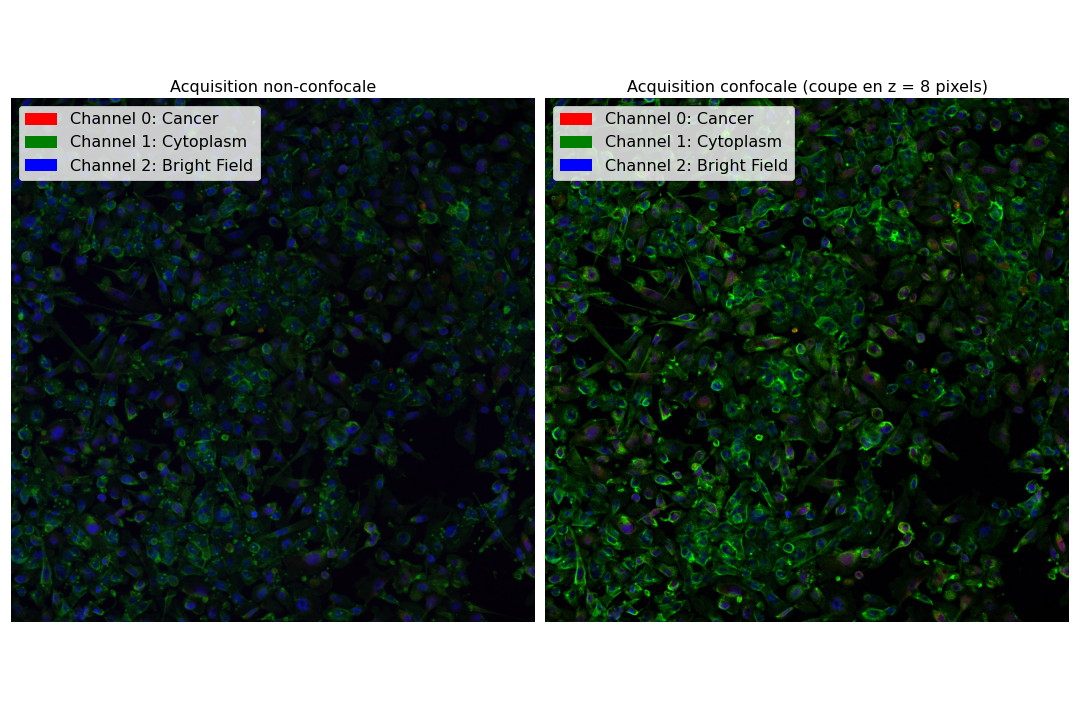
\includegraphics[scale=0.45]{non_and_yes_confocal.png}
  \caption{Comparaison de l'imagerie obtenue d'un système non-confocal (à gauche) à celle d'un système confocal (à droite).}
  \label{non_yes_confo}
\end{figure}

Il est possible de voir une meilleure résolution sur l'acquisition confocale, ce qui résulte en des contours plus définis. Ensuite, la figure \ref{3d_cells} présente trois coupes de l'image 3D autour du même point dans l'espace afin de
représenter le volume de quelques cellules.

\begin{figure}[H]
  \centering
  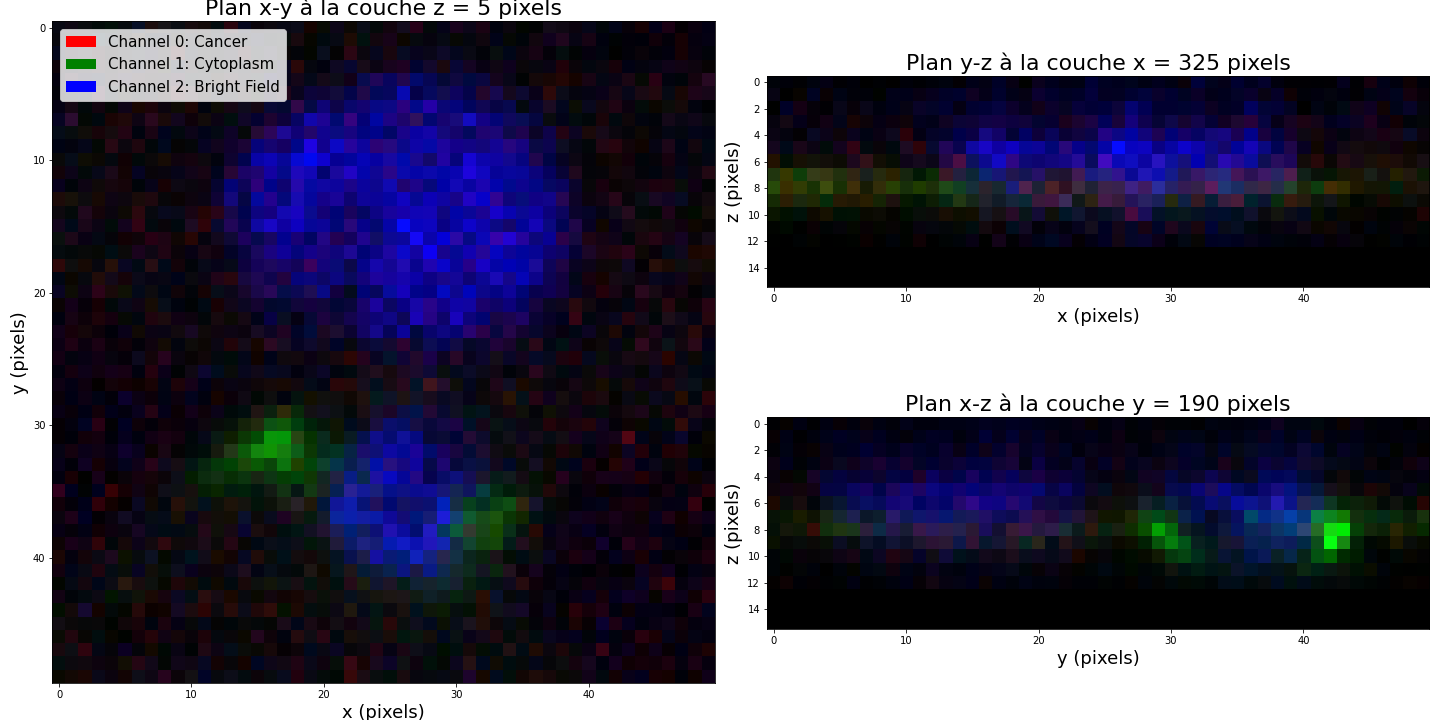
\includegraphics[scale=0.34]{volume.png}
  \caption{Volume de deux cellules bien visibles par LSCM en fluorescence présenté en trois plans.}
  \label{3d_cells}
\end{figure}


\section{Discussion}

\subsection{Retour sur l'hypothèse}

Trois hypothèses ont été posées lors du rapport préliminaire : la résolution axiale augmente linéairement en fonction de la taille du sténopé, la résolution axiale augmente de façon quasi-linéaire en fonction de la longueur focale des lentilles et la résolution reste inchangée peu importe l'espace entre les lentilles.

La première de ces trois hypothèses peut être vérifiée en se basant sur les deux cas extrêmes étudiés lors du laboratoire. Dans l'un, le sténopé vient contraindre la lumière incidente et, dans l'autre, son absence peut être interprétée comme un sténopé de diamètre suffisamment large pour ne plus être l'ouverture d'arrêt du système, laissant passer toute la lumière incidente. Les résultats obtenus et présentés dans les figures \ref{fit 1} et \ref{fit 2} valident cette hypothèse. La largeur à mi-hauteur étant plus grande sans sténopé, ou en d'autre termes, la première hypothèse, soit : la résolution axiale augmente linéairement en fonction de la taille du sténopé. Néanmoins, le caractère linéaire de cette évolution n'a pas pu être explicitement représentées lors du laboratoire. En effet, l'étude de ces deux cas extrêmes ne permet qu'une seule conclusion : la résolution augmente avec la taille du sténopé, sans pour autant en détailler le comment. D'autant plus que lorsque le sténopé n'est plus l'ouverture d'arrêt, la résolution finit par rester constante, car sa dépendance n'est maintenant qu'à l'alignement du reste du système.

Pour ce qui est des deux autres hypothèses, elles n'ont pas pu être explicitement validées ou réfutées lors du laboratoire. Notamment, par exemple, la deuxième hypothèse pourrait être, pour certaines valeurs de distance focale, interprétée comme un système sans sténopé, mais où le point observateur serait décalé. Elles auraient nécessité une étude plus explicite lors du laboratoire, car elle ne reste ici que sources d'interprétation et non de faits. 

\subsection{Analyse des causes d'erreurs}

Les erreurs liées aux données récoltés trouvent leur causes dans de nombreux éléments du systèmes optiques et des différents procédés d'analyse. A commencer par les incertitudes relatives aux appareils de mesure utilisés. Les figures \ref{brutes 1} et \ref{brutes 2} représentent comme présenté en partie 1 les résultats de mesures obtenues pour les deux systèmes, elles permettent aussi de mettre en évidence les erreurs relatives à chaque mesures. Erreurs liées aux échelles de mesures de la monture de translation pour les barres horizontales et celles du power-meter pour les barres verticales. Le tableau \ref{incertitudes} présente les incertitudes de chacun de ces composant optiques. 

\begin{table}[H]
\centering
\begin{tabular}{|p{4.8cm}|p{4.2cm}|}
\cline{2-2}
\multicolumn{1}{c|}{} & \textbf{Incertitude} \\
\hline
\textbf{Monture de translation} & 10 microns\\
\hline
\textbf{Power-Meter} & 2.61\\
\hline
\end{tabular}
\caption{Incertitudes sur les mesures de la monture de translation et du power-meter}
\label{incertitudes}
\end{table}

L'incertitude de 10 microns liée à la monture de translation est donné par le constructeur du dispositif. Dans le cas du power-meter, ces erreurs ont été calculées en prenant les valeurs maximales, minimales et moyenne des données recueillis, puis en faisant une moyenne des écarts à gauche et à droite.

De plus, sur chacun des graphiques obtenus, un autre maximum d'amplitude se dessine, révélé par les courbes gaussiennes de couleur jaune. Le fait que ces deux anomalies soient présentent quelque soit le jeu de données indique une défaillance au niveau de la source de lumière du système, du laser. C'est cette défaillance qui oblige à utiliser une somme de courbe gaussienne et qui induit donc des erreurs lors de l'estimation de la résolution. De façon générale, l'utilisation de librairies comme \textit{lm.fit} induit des sources d'erreurs lors de l'étude d'un jeu de données discret. Mais le fait de devoir sommer des courbes gaussiennes en les considérant adéquates, force à relier la résolution estimée à une solution qui ne la représente que indirectement (la courbe bleu du jeu de données avec sténopé n'étant pas exactement la courbe représentative du système dans un cas idéal).

D'autres erreurs, plus pratiques, liées à l'alignement du système sont aussi à noter. Notamment lors des étapes d'alignement des back réflections. Néanmoins, le suivit en temps réel des valeurs de puissance recueillis à permit d'ajuster l'alignement du sténopé et ainsi maximiser l'amplitude du système. 

\subsection{Question 1}
%TODO
Le fonctionnement de base de la microscopie confocale par fluorescence repose sur l'utilisation de la fluorescence afin de visualiser des points spécifiques de l'échantillon \cite{elliott_confocal_2020}. En d'autres termes, l'échantillon est balayé, point par point, par un laser focalisé dans le but de produire les différentes profondeurs de l'image. Les fluorophores placés à certains points de l'échantillon sont alors excités par le faisceau laser, produisant une fluorescence. Cette lumière passe, ensuite, dans le sténopé, permettant l'élimination des rayons lumineux hors-focus, et est détectée par le capteur; l'image est, ainsi, créée.

Les couleurs des images dans la microscopie LSCM par fluorescence proviennent des fluorophores utilisés pour marquer les points de l'échantillon. Ces fluorophores correspondent à des protéines fluorescentes qui ont deux longueurs d'ondes importantes : la longueur d'onde d'absorption et la longueur d'onde d'émission. Les protéines, lorsqu'elles absorbent la lumière, émettent une lumière à une longueur d'onde supérieure à celle absorbée. De ce fait, lorsque l'échantillon est balayé par le laser, les fluorophores excités retransmettre une lumière à une certaine longueur d'onde. Celle-ci est, ensuite, captée par le détecteur et crée ainsi la gamme de couleurs retrouvées \cite{leclerc_proteines_2014}. Comme ces protéines sont fabriquées spécialement pour se joindre à des parties spécifiques des cellules, la fluorescence permet l'observation ciblée de différents éléments de la matière observée, à l'aide de canaux différents.

En ce qui a trait aux différents canaux de l'image, le premier canal correspond aux cellules cancéreuses de l'échantillon, soit les parties anormales à détecter. Le deuxième canal correspond au cytoplasme, soit la partie gélatineuse du contenu de la cellule. Celle-ci se trouve entre la membrane plasmique et le noyau \cite{futura_definition_2024}. Finalement, le dernier canal de l'image correspond au \textit{bright field}. Ce canal représente une image en lumière blanche traditionnelle, la lumière est transmise à travers l'échantillon et le contraste est généré par l'absorption de celle-ci dans les zones denses. Donc, ce canal permet d'offrir une visualition générale de la cellule \cite{sciencedirect_bright_nodate}.

\subsection{Question 2}
Pour trouver une estimation de la résolution du système, la taille réelle d'une cellule cancéreuse de prostate est d'abord trouvée. De cette manière, le diamètre d'une cellule réelle est d'environ 16.6$\pm$2.9 $\mu$m avec une épaisseur d'environ 15.1$\pm$2.6 $\mu$m \cite{seo_mechanical_2017}. Ensuite, à partir de l'image 3D donnée, le nombre de pixel pour le diamètre de de la cellule est évaluée. Donc, pour la cellule sur la figure \ref{3d_cells}, un diamètre d'environ 25$\pm$1 pixels et une épaisseur de 12$\pm$1 sont comptés. Avec ces données, il est possible de calculer la résolution latérale et axiale. Donc, la résolution est donnée par l'équation suivante :
\begin{equation}
  R=\frac{\text{Diamètre de cellule réelle}}{\text{Nb de pixels}}
\end{equation}
La résolution latérale correspond au plan \textit{xy}, ainsi le résultat de celle-ci est de :
\begin{equation}
  R_{L}=\frac{16.6\,\mu\mathrm{m}}{25\,\mathrm{Pixels}}=0.66\,\frac{\mu\mathrm{m}}{\mathrm{Pixels}}
\end{equation}
En utilisant la même équation pour la résolution axiale, correspondant au plan \textit{z}, le résultat obtenu est de :
\begin{equation}
  R_{A}=\frac{15.1\,\mu\mathrm{m}}{12\,\mathrm{Pixels}}=1.3\,\frac{\mu\mathrm{m}}{\mathrm{Pixels}}
\end{equation}
Pour les deux valeurs obtenues, les incertitudes sont calculées à l'aide de la formule suivante :
\begin{equation}
  \Delta R=\sqrt{\left(\frac{\Delta V_{R}}{V_{R}}\right)^{2}+\left(\frac{\Delta V_{P}}{V_{P}}\right)^{2}}
\end{equation}
Où $\Delta V_{R}$ est l'incertitude de la valeur réelle de la cellule, $V_{R}$ est la valeur réelle de la cellule, $\Delta V_{P}$ est l'incertitude de la valeur comptée, et $V_{P}$ est la valeur comptée. Ainsi, les valeurs estimées de résolution avec leur incertitude sont les suivantes :
\begin{align*}
  R_{L}&=0.66\pm0.2\,\mu\mathrm{m} & R_{A}&=1.3\pm0.2\,\mu\mathrm{m} \\
\end{align*}

\subsection{Question 3}
Le rôle d'un sténopé dans un système optique est d'éliminer les faisceaux lumineux ne provenant pas du plan focal, permettant d'améliorer la définition et la netteté des images. Cependant, la taille de ce diaphrame est important dans le balancement de la résolution et de la quantité de lumière admise par le système. En effet, si la taille du sténopé est trop petite, la quantité de lumière provenant du plan focal lui-même est réduite, engendrant une perte de puissance. De plus, puisque la quantité de lumière atteignant le détecteur est réduite, le rapport entre le bruit et les signaux diminue, ce qui rend le bruit de fond plus apparent. De cette manière, les images peuvent apparaître moins définies et plus sombres \cite{semwogerere_confocal_2005}. 

Par exemple, pour un système parfait utilisant un profil de faisceau gaussien et opérant à une longueur d'onde de 600 nm, la taille du sténopé le plus petit qu'il serait possible d'utiliser peut être calculée à l'aide de la formule suivante \cite{noauthor_gaussian_2024} :
\begin{equation}
  \theta=\frac{\lambda}{n\pi\omega_{0}}
\end{equation}
Où $\lambda$ est la longueur d'onde, soit de 600 nm, $\omega_{0}$ est la taille du faisceau, et $n$ est l'indice de réfraction. La taille du sténopé peut être estimée à partir de la taille du faisceau. En effet, dans un système parfait, la taille du faisceau est approximativement proportionnelle à celle du sténopé. Donc, pour trouver la valeur de $\omega_0$, il faut estimer la valeur de l'angle de divergence du faisceau. Pour trouver cet angle, l'angle de convergence de la dernière lentille est calculé.
\begin{equation}
  \theta=2\tan\left(\frac{\phi/2}{f}\right)
\end{equation}
En utilisant les valeurs numériques données dans le procédurier, un angle de 0.7 radians est trouvé. Ainsi, en isolant la valeur recherchée dans l'équation 5 et en calculant numériquement, la taille la plus petite pour le sténopé est de :
\begin{equation}
  \omega_{0}=\frac{\lambda}{n\pi\theta}=272.84\,\mathrm{nm}
\end{equation}

\subsection{Question 4}
La résolution latérale correspond à la capacité d'un système à distinguer les points d'un objet qui sont situés à proximité l'un de l'autres alors que le contraste, étroitement lié à la résolution, est défini comme la quantité de photons collectés à partir de l'échantillon \cite{spring_confocal_nodate}. Les systèmes confocaux permettent d'améliorer ces deux paramètres avec l'ajout d'un diaphrame optique. Comme mentionné, l'ajout de ce sténopé permet de limiter les faisceaux lumineux, ce qui élimine les rayons en provenance des plans non-focaux. Puisque la lumière atteignant le détecteur ne provent que du plan focal de l'échantillon, le bruit créé par les rayons extérieurs est réduit. De cette manière, le flou créé par ces rayons est éliminé et la différence de lumiosité entre les structures est mieux définie, offrant ainsi une amélioration dans la résolution et dans le contraste \cite{borlinghaus_pinhole_2017}.

Par exemple, dans la figure \ref{3d_cells} utilisant le système confocal, il est possible d'observer, en ce qui a trait au contraste, que des différences de lumiosité entre les canaux. En effet, les détails des divers canaux, soient le rouge, le bleu et le vert, peuvent être distingués clairement les uns des autres. Cependant, dans le cas de celui qui n'utilise pas le système confocal, soit le suivant :
\begin{figure}[H]
  \centering
  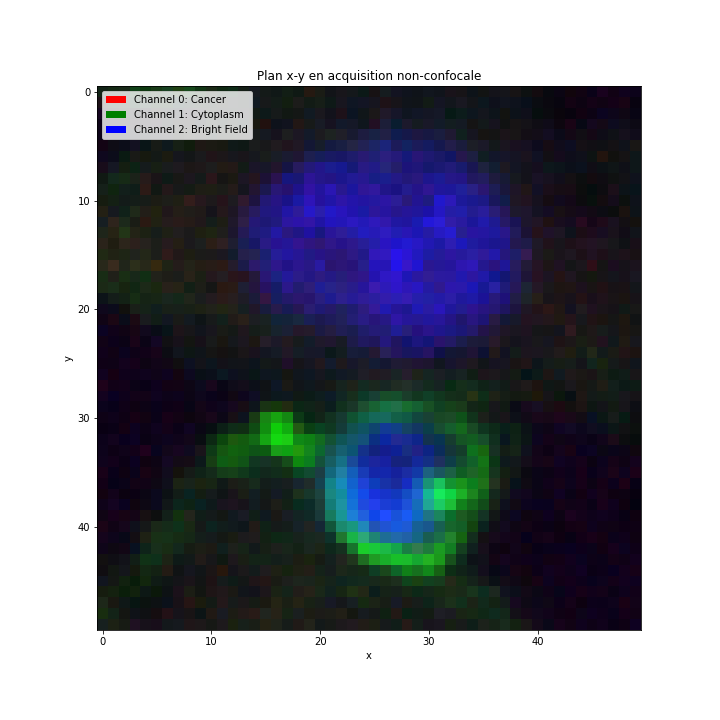
\includegraphics[scale=0.35]{xy_plane_non_confocal.png}
  \caption{Image de la cellule sans le système confocal.}
  \label{non-confocal}
\end{figure}
Les détails sont légèrement moins marqués que pour ceux de la figure \ref{3d_cells}, particulièrement dans les zones où les couleurs se chevauchent. De plus, pour l'image confocale, celle est mieux définie avec des contours plus nets autour des structures, facilitant la distinction des composantes. Ainsi, avec ces exemples, il est possible de visualiser l'augmentation de la résolution et du contraste lorsqu'un système confocal est utilisé.

Bien que les systèmes confocaux font preuve de plusieurs avantages, ceux-ci comportent quelques désavantages. Un premier désagrément est la vitesse d'acquisition des données. Puisque les points sont balayés individuellement, l'acquisition des données est trop lente pour obtenir des informations sur des systèmes biologiques rapide \cite{st_croix_confocal_2005}. De plus, les microscopes confocaux n'utilisent qu'un seul photon pour exciter les fluorophores, ce qui peut résulter à plus grande dispersion de la lumière dans l'image que, par exemple, des sytèmes multiphotoniques \cite{francis_confocal_2023}.

\section{Conclusion}
En conclusion, l'objectif de cette expérience consistait à mesurer la résolution axiale d'un système confocal à travers l'analyse d'une courbe d'intensité axiale d'un système avec et sans l'utilisation d'un sténopé. De cette manière, après avoir amassées les données d'intensité, des courbes de tendance ont pu être créées. À partir des courbes d'intensité, l'amplitude représentative de la résolution a pu être calculée à l'aide de la largeur à mi-hauteur de la valeur maximale. Cette estimation de la largeur a permis d'offrir les résultats approximatifs de la résolution. Pour justifier les divergences entre les hypothèses théoriques précédentes, quelques causes d'erreur ont été notées telles que les incertitudes relatives aux appareils, une défaillance au niveau de la source lumineuse, et l'alignement du système. Or, malgré la légère divergence de résultat, l'expérience a permis de visualiser l'influence d'un sténopé dans la limitation des faisceaux non-focaux et l'amélioration de la qualité d'imagerie, offrant ainsi des perspectives intéressantes sur les techniques d'imagerie de performance et un approfondissement des connaissances en optique, autant pratiques que théoriques.


\clearpage


\bibliographystyle{unsrtnat}
\bibliography{microscopie_final.bib}

\end{document}
